\documentclass[12pt,french,titlepage]{article}
\author{par Léo Peyronnet}
\title{sim-rhinite\\[1ex] \large Projet Informatique L2}
\date{Juin 2024}

% Package langue
\usepackage{babel}

% Package liens
\usepackage{hyperref}

% Package graphiques et images
\usepackage{graphicx} 
\usepackage{float}

% Police principale
\usepackage{mathptmx}

% Marges
\usepackage[margin=1in]{geometry}

% Interligne de 1,5
\usepackage{setspace}
\onehalfspacing

% Définition couleur pour commentaires code
\usepackage{xcolor}
\definecolor{ao(english)}{rgb}{0.0, 0.5, 0.0}

% Portions de code en police Courier
\usepackage{courier}
\usepackage{listings}
\lstset{
  basicstyle=\ttfamily\footnotesize, % Police Courier taille 10
  breaklines=true,
  extendedchars=true,
  commentstyle=\color{ao(english)},
  breaklines=true,
  keywordstyle=\color{blue},
  language=C,
  literate=
  {²}{{\textsuperscript{2}}}1
  {⁴}{{\textsuperscript{4}}}1
  {⁶}{{\textsuperscript{6}}}1
  {⁸}{{\textsuperscript{8}}}1
  {€}{{\euro{}}}1
  {é}{{\'e}}1
  {è}{{\`{e}}}1
  {ê}{{\^{e}}}1
  {ë}{{\¨{e}}}1
  {É}{{\'{E}}}1
  {Ê}{{\^{E}}}1
  {û}{{\^{u}}}1
  {ù}{{\`{u}}}1
  {â}{{\^{a}}}1
  {à}{{\`{a}}}1
  {á}{{\'{a}}}1
  {ã}{{\~{a}}}1
  {Á}{{\'{A}}}1
  {Â}{{\^{A}}}1
  {Ã}{{\~{A}}}1
  {ç}{{\c{c}}}1
  {Ç}{{\c{C}}}1
  {õ}{{\~{o}}}1
  {ó}{{\'{o}}}1
  {ô}{{\^{o}}}1
  {Õ}{{\~{O}}}1
  {Ó}{{\'{O}}}1
  {Ô}{{\^{O}}}1
  {î}{{\^{i}}}1
  {Î}{{\^{I}}}1
  {í}{{\'{i}}}1
  {Í}{{\~{Í}}}1,
}

\begin{document}

\maketitle

\tableofcontents
\newpage

\section{Projet de simulation}
Ce projet s'inscrit dans l'évaluation d'un enseignement dispensé en L2 Informatique par l'UCA nommé "Projet Informatique". Cet enseignement a pour sujet la \textbf{réalisation de simulations scientifiques à l'aide d'outils informatiques}. Ce projet répond au sujet de session de rattrapage de l'année 2024.  

\subsection{Présentation de la simulation et de ses objectifs}
\label{sec:objectifs}
\textbf{sim-rhinite} est un projet de simulation de maladie infectieuse type rhinite. L'objectif principal de cette simulation est de modéliser la propagation d'un virus non mortel dans une population et de produire des statistiques à partir de ce modèle qui pourront être analysées ultérieurement.
Les objectifs spécifiques de cette simulation sont les suivants :

\begin{enumerate}

\item \textbf{Modélisation la population et l'espace de simulation}
\begin{itemize}
\item Création d'une grille 2D torique pour représenter l'espace dans lequel les individus se déplacent.
\item Initialisation d'une population avec des positions aléatoires sur cette grille.
\end{itemize}

\item \textbf{Dynamique de déplacement}
\begin{itemize}
\item Simulation du déplacement aléatoire des individus sur la grille, de 6h à 22h chaque jour, avec un pas de temps d'une heure.
\end{itemize}

\item \textbf{Propagation et évolution du virus}
\begin{itemize}
\item Implémentation des règles de propagation du virus avec une probabilité de transmission dépendant de l'état de la maladie chez l'individu infecté et de son voisinage de Moore d'ordre 2.
\item Modélisation de la période d'incubation et les différentes phases de contagiosité du virus sur une période de 12 jours.
\end{itemize}

\item \textbf{Variables}
\begin{itemize}
\item Initialisation de la simulation avec différents nombres de personnes contaminées (de 1 à 10) afin d'observer les effets sur la propagation.
\end{itemize}

\item \textbf{Statistiques}
\begin{itemize}
\item Les simulations sont répétées 30 fois pour chaque valeur de notre variable d'expérience (nombre initial de contaminés).
\item Les résultats sont collectés et présentés sous forme de tableaux avec des intervalles de confiance à 95\%.
\end{itemize}

\end{enumerate}
 
\subsection{Choix conceptuels}
\subsubsection{Constante temporelle}
Dans le sujet, il est demandé de tester la simulation sur 1 mois, 3 mois, 6 mois et 1 an. Il est alors possible de faire de la durée de simulation une seconde variable de notre expérience afin de produire des statistiques pour chaque combinaison de valeurs de variables (durée et nombre initial de contaminés). Cependant, les informations des simulations sur 1, 3 et 6 mois sont également contenues dans la simulation sur 1 an. 

Soit $1,2,6$ et $12$ des ensembles représentant les informations récoltées lors d'une simulation de durée égale à leur symbole (en mois), alors :
$$
1 \subset 3 \subset 6 \subset 12
$$

Il n'est alors nécessaire de simuler qu'avec la durée maximale, c'est à dire 1 an (12 mois). Nous pouvons donc considérer la durée comme une constante.

\subsubsection{Positionnement de la population}
Dans le sujet, il est indiqué que l'on positionne sur la grille les personnes avec des coordonnées aléatoires. Cependant, rien n'est explicité dans le cas où deux personnes obtiennent les mêmes coordonnées. J'ai donc jugé bon que les coordonnées soit unique à une personne.

\subsubsection{État de la personne au terme de la contamination}
Dans le sujet, rien n'est explicité quant à l'état d'une personne contaminée lorsqu'elle arrive au terme de sa période de contamination (j+12). Est-elle considéré comme à nouveau saine (et donc contaminable) ou considérons nous qu'elle est "guérie", c'est à dire immunisée à la maladie et donc non contaminable ? 

Suite à la consultation du responsable de l'enseignement, un compromis a été décidé. Au terme de sa période de contamination, la personne est considérée comme guérie pendant une durée établie, puis au terme de cette dernière, la personne est reconsidéré comme saine (et donc contaminable).

Nous reviendrons ultérieurement sur le choix de valeur de cette durée d'immunité (cf. \ref{sec:analyse}).

\newpage



\section{Programme informatique}
La simulation a été implémentée par un programme écrit en langage C. Le répertoire du projet est disponible sur un dépôt distant, fourni en annexe.


\subsection{Choix d'implémentation}
\subsubsection{Générateur d'aléatoire}
Dans le sujet, il est demandé d'utiliser “le meilleur générateur de nombre pseudo-aléatoire vu en cours”. Conformément à ce que l'on a vu en cours et en TP, j'ai choisi le \textbf{Mersenne Twister} dans son implémentation MT 19937. Ainsi, dans la suite de cette rédaction, tous les appels à l'aléatoire sont à comprendre comme des appels à ce générateur.

\subsubsection{Format des résultats finaux}
Le programme doit produire des données statistiques sur la simulation. J'ai choisi le format \textbf{CSV} pour stocker ces résultats, notamment pour ma familiarité avec ce format, sa simplicité et la possibilité d'être lu facilement par les outils que j'ai utilisé pour la création de visuels (cf. \ref{sec:script_graph}).

Les fichiers ainsi crées par le programme seront placés dans un répertoire spécial situé à la racine et nommé \textbf{out/}.


\subsection{Structure du projet}


Le projet est composé de deux programmes exécutables :

\begin{itemize}
\item \textbf{stats\_sim} : Il permet de produire des statistiques sur l'évolution de la contamination de la maladie en fonction du nombre d'infectés initiaux.
\item \textbf{idle} : Annexe permettant de visualiser le comportement de la population simulée.\\
\end{itemize}



Le répertoire racine du projet comprend plusieurs sous-répertoires :
\begin{itemize}
\item \textbf{redaction/} : comprend l'ensemble des fichiers relatif à ce compte-rendu.
\item \textbf{source/} : comprend l'ensemble des fichiers sources du programme.
\item \textbf{packages/} : comprend l'ensemble des dépendances logicielles du programme.
\end{itemize}

La racine contient également un builder et un fichier \textbf{README.md} contenant des informations sommaires sur le projet et des consignes d'usage.

\newpage
 
\subsubsection{Packages employés}
Le sous-répertoire \textbf{packages/} contient :
\begin{itemize}
\item \textbf{affichage/} : fonctions d'affichage de tableau et de matrices.
\item \textbf{csv/} : fonction d'écriture de matrices au format CSV.
\item \textbf{menuing/} : ensemble de fonctions permettant la création, la gestion et l'affichage de menus dynamiques dans le terminal.
\item \textbf{mt19937ar/} : fonctions relatives à la génération de nombres pseudo-aléatoires selon le Mersenne Twister. 
\end{itemize}

\subsubsection{Code source et builder}
Les fonctions (fonctions métier, initialisation et fonction launch\_sim) ainsi que les structures de données communes aux deux programmes sont définies dans le fichier source \textbf{rhinite.c} et son fichier d'en-tête \textbf{rhinite.h}. Ensuite, chaque programme possède son propre fichier source qui fait appel à \textbf{rhinite.h}.

Comme expliqué précédemment, le projet est équipé d'un builder (\textbf{makefile}) qui facilite le processus de compilation des fichiers sources du projet mais aussi des différents packages. Les informations relatives à son utilisation sont disponibles dans le fichier \textbf{README.md} mentionné précédemment.


\subsection{Structuration des données}
\label{sec:struct_donnees}
Le fichier \textbf{rhinite.h} défini deux types personnalisés :
\begin{itemize}
\item \textbf{etat\_t} : énumération des états dans lesquels une personne pourra être. Défini un état sain, incubant, contaminant et guéri.
\begin{lstlisting}
typedef enum {SAIN, INCUBANT, CONTAGIEUX, GUERI} etat_t;
\end{lstlisting}

\item \textbf{personne\_t} : structure représentant un individu (ou personne) d'une population. Composée d'un couple d'entiers représentant la position de la personne sur la grille, d'un état comme défini au-dessus et d'un autre entier comptant le nombre de jours depuis que la personne est infectée.
\begin{lstlisting}
typedef struct {
    int x, y;
    etat_t etat;
    int jour_infection;
} personne_t;
\end{lstlisting}
\end{itemize}

Une population pourra ainsi être représentée par un tableau de personne. 

\subsection{Fonctions d'initialisation}
Le fichier \textbf{rhinite.c} permet l'initialisation d'une population grâce à une fonction nommée \textbf{init\_population}. Cette fonction permet donc l'initialisation d'une population, induisant qu'elle fourni à ses individus des coordonnées aléatoires uniques. La fonction retourne un tableau de n personnes.

Une autre fonction nommée \textbf{init\_contamination} permet de définir dans une population les individus qui seront les infectés initiaux. Pour rappel, leur nombre correspond à notre variable d'expérience (cf. \ref{sec:objectifs}). La sélection de ces individus parmi la population se fait de manière aléatoire.   


\subsection{Fonctions métiers}
Le fichier \textbf{rhinite.c} implémente également plusieurs autres fonctions permettant de manipuler une population.

\subsubsection{deplacement\_alea}
\textbf{deplacement\_alea} permet de déplacer chaque individu vers une case adjacente à la sienne. Cette case est choisie de manière aléatoire parmi celles qui ne sont pas occupées par un autre individu de la population. Les coordonnées des individus leurs sont donc ainsi toujours uniques. Aussi, si toutes les cases adjacentes sont occupées, le déplacement est annulé.

La fonction prends également en compte le fait que la grille sur laquelle les individus sont placés est torique.



\subsubsection{evolution\_journaliere\_maladie}
\textbf{evolution\_journaliere\_maladie} permet de faire évoluer l'état de la maladie pour chaque individu infecté. Elle incrémente donc le compteur \textbf{jour\_infection} (cf. \ref{sec:struct_donnees}) pour tous les individus infectés. Elle gère ensuite leur changement d'état en fonction des durées de chacun des états de la maladie. 

\subsubsection{contamination}
\textbf{contamination} gère les contaminations entre les individus. Pour chaque individu contagieux, elle réalise un lancer aléatoire pour chaque autre individu présent dans le voisinage de Moore d'ordre 2 de l'individu contagieux. 

La probabilité de contamination est définie de manière discrète en fonction de la valeur de \textbf{jour\_infection}. Ainsi, si le lancer possède une valeur inférieure ou égale à la probabilité de contamination, l'individu voisin est infecté.

Cette fonction comptabilise également le nombre de contaminations réalisées durant son appel (qui correspond à une heure dans le contexte de notre simulation). Cette comptabilisation sert de base pour le travail d'analyse statistique que nous verrons ultérieurement. \textbf{contamination} renvoie donc un entier représentant cette comptabilisation.

\subsection{Fonction launch\_sim}
La fonction \textbf{launch\_sim} permet de réaliser une simulation complète suivant des paramètres donnés et fait appel à l'ensemble des fonctions présentées précédemment. Elle permet notamment de leur apporter un contexte temporel. 

Ainsi, elle commence par faire appel aux fonctions d'initialisation ; d'abord \textbf{init\_population} qui lui renvoie un tableau de personnes, puis \textbf{init\_contamination} qui prend, entre autres paramètres, ce tableau.

Ensuite, pour chaque jour prévu dans la simulation, elle lance un cycle de 24 heures à l'intérieur duquel, pour chaque heure, est fait appel à la fonction \textbf{contamination}, et si l'heure est comprise entre 6 heures et 22 heures, un appel à la fonction \textbf{deplacement\_alea}.

Enfin, au terme de chaque jour, la somme des contaminations qui ont eu lieu dans la journée est stockée dans un tableau d'entiers initialisé au préalable et un appel à  \textbf{evolution\_journaliere\_maladie} est effectué pour mettre à jour les états journaliers.

\textbf{launch\_sim} se clôt en revoyant le tableau de contamination journalière, ayant donc une taille égale au nombre de jours compris par la simulation.

\newpage

\subsection{Programmes exécutables}
\subsubsection{stats\_sim}
\label{sec:stats_sim}
Le programme \textbf{stats\_sim} fait appel à \textbf{launch\_sim} afin de produire des statistiques sur l'évolution de la contamination de la maladie en fonction du nombre d'infectés initiaux.

Après avoir initialisé le générateur de pseudo-aléatoire, le programme initialise et défini l'ensemble des variables et constantes du programme :
\begin{lstlisting}
// Déclaration constantes programme
    double        proba_contamination[12]   = {0, 0, 0, 0.6, 0.8, 0.7, 0.6, 0.5, 0.4, 0.3, 0.2, 0.1};
    int           duree_incubation          = 2; // en jours
    int           duree_contagion           = 9; // en jours
    int           jours                     = 365; // un an de simulation
    int           nb_replications           = 30;

    // Déclarations variables programme (constantes expérience)
    int           taille_grille;
    int           num_personnes;
    int           duree_immunite; // en jours

    // Déclaration variable programme (variable expérience)
    int           num_infect_init;
    
    // Initialisation constantes expérience
    taille_grille     = 50;
    num_personnes     = 100;
    duree_imunitee    = 15;
\end{lstlisting}

Les valeurs présentées ici représentent les valeurs par défaut du programme et correspondent à celles indiquées dans le sujet. Nous appellerons désormais cette collection de valeurs "\textbf{default}" et elle servira de base dans notre travail d'analyse (cf. \ref{sec:analyse})\\

Ensuite, le programme boucle pour chaque valeur de \textbf{num\_infect\_init} de 1 à 10 (inclus). Pour chaque itération de la boucle, une seconde boucle est définie. Son nombre d'itération est égal à la valeur de \textbf{nb\_replications} (dans notre cas, 30). 

Ainsi, pour chaque itération de la seconde boucle, un appel à \textbf{launch\_sim} est effectué et le tableau retourné par cette dernière est stocké dans un tableau de pointeurs initialisé en amont. Au terme de la seconde boucle, le tableau de pointeurs contient donc 30 tableaux d'entiers qui contiennent chacun $j$ entiers, avec $j$ la durée de la simulation exprimée en jours (cf. constante \textbf{jours}).


Le programme exploite ce tableau de pointeur pour réaliser des calculs statistiques. Pour chaque jour, il calcule le nombre de contamination moyen des 30 réplications, leur écart-type et à partir de cela, un intervalle de confiance à 95\%. L'intervalle est stocké dans un second tableau ayant une taille égale à $j$.

Enfin, le programme inscrit ce tableau d'intervalles dans un ficher formaté CSV avec un nom indiquant la valeur de \textbf{num\_infect\_init} avec laquelle la simulation a tournée. Ceci conclu une itération de la première boucle. Une fois cette dernière finie, le programme se termine.

\subsubsection{idle}
Le programme \textbf{idle} est une annexe permettant de visualiser le comportement de la population simulée. Il utilise une fonction nommée \textbf{launch\_idle} qui correspond à une "redéfinition" de la fonction \textbf{launch\_sim} auquel des affichages dans le terminal ont été ajoutés.\\

\textbf{idle} démarre avec un menu donnant à l'utilisateur le choix entre plusieurs modes de lancement du programme :
\begin{itemize}
\item Vérification collisions : lance une simulation de un seul jour dans une grille minime (2x2) afin de visualiser le fonctionnement de la fonction métier \textbf{deplacement\_alea} et sa gestion des "collisions" entre les individus.

\item Valeurs par défaut : lance une simulation réduite par rapport à celle effectuée dans \textbf{launch\_sim}. La durée de la simulation est de 15 jours, dans une grille 30x30 avec 50 personnes, dont 5 sont des infectés initiaux. Cette simulation permet d'avoir une vue plus globale du comportement d'une population tel que décrit par les fonctions métiers.\\
\end{itemize}

Pour gérer l'affichage de la grille, \textbf{idle} défini trois fonctions :
\subsubsection*{comparer\_personnes}
Cette fonction de comparaison est utilisée par la fonction \textbf{qsort} pour trier un tableau de structures personne\_t. Elle prend en entrée deux pointeurs génériques a et b, qu'elle convertit en pointeurs de type personne\_t.

Elle compare d'abord les coordonnées x des deux personnes. Si elles sont différentes, la fonction retourne la différence entre ces deux coordonnées, ce qui permet de les trier en ordre croissant de x. Si les coordonnées x sont égales, la fonction compare alors les coordonnées y de manière similaire. Ainsi, les personnes sont triées d'abord par leur position x, puis par leur position y en cas d'égalité sur x.

\subsubsection*{tri\_croiss\_population}
Cette fonction prend un tableau de structures personne\_t et le nombre d'éléments dans ce tableau. Elle alloue de la mémoire pour une copie de ce tableau, vérifie si l'allocation est réussie, et copie chaque élément du tableau original dans la copie.

Ensuite, elle utilise la fonction \textbf{qsort} pour trier la copie du tableau en utilisant la fonction de comparaison \textbf{comparer\_personnes}. La fonction retourne finalement le pointeur vers la copie triée du tableau.

\subsubsection*{affich\_population}
Cette fonction affiche la population sur une grille de taille \textbf{taille\_grille}. Elle commence par trier la population en utilisant la fonction \textbf{tri\_croiss\_population} et stocke le résultat dans \textbf{population\_ordone}.

Ensuite, elle affiche une bordure supérieure en utilisant le caractère '\#'. Pour chaque ligne de la grille, elle affiche également une bordure latérale gauche, puis vérifie pour chaque colonne si une personne de la population triée occupe cette position (c'est à dire que les coordonnées x et y correspondent à celles de la grille). Si une personne est présente, son état est affiché ; sinon, un espace vide est affiché. Après chaque ligne de la grille, une bordure latérale droite est affichée.

Finalement, une bordure inférieure est affichée. La fonction libère ensuite la mémoire allouée pour la copie triée de la population.

\newpage

\section{Analyse des résultats}
\label{sec:analyse}

Cette partie rassemble mes analyses sur certains résultats de simulations que j'ai produit avec \textbf{stats\_sim}. Les représentations visuelles de ces résultats ont été obtenu grâce à un script dont je détaille le fonctionnement en annexe (cf. \ref{sec:script_graph}). 

\subsection{Présentation des simulations}
Commençons cette analyse par une définition des différentes simulations sélectionnées :
\begin{itemize}
\item \textbf{default} : correspond au valeurs de constantes d'expérience par défaut du programme \textbf{stats\_sim} (cf. \ref{sec:stats_sim}).
\begin{itemize}
\item taille\_grille = 50
\item num\_personnes = 100
\item duree\_imunite = 15
\end{itemize}

\item \textbf{default-sans-imunite} : correspond à la simulation \textbf{default} dont la valeur de duree\_imunitee est nulle.


\item \textbf{default-duree-immunite-10} : correspond à la simulation \textbf{default} dont la valeur de duree\_imunitee a été abaissée à 10.

\item \textbf{default-duree-immunite-10-replic-300} : correspond à la simulation \textbf{default-duree-immunite-10} dont le nombre de réplications a été multiplié par 10.\\


\item \textbf{max} : correspond à la plus grosse simulation effectué.
\begin{itemize}
\item taille\_grille = 100
\item num\_personnes = 500
\item duree\_imunite = 15
\end{itemize}

\item \textbf{max-duree-imunite-30} : correspond à la simulation \textbf{max} dont la valeur de duree\_imunitee a été augmentée à 30.

\end{itemize}

\newpage

\subsection{Vagues de contamination}

Au travers des résultats des simulations \textbf{default-duree-immunite-10}, \textbf{default-sans-immunite} et \textbf{max}, il est possible d'observer une ondulation des courbes représentatives de l'intervalle de confiance du nombre de contamination par jour. (cf. fig. \ref{fig:default-duree-immunite-10-num_infect_init_1}, \ref{fig:default-sans-immunite-num_infect_init_1} et \ref{fig:max-num_infect_init_1})\\

La période de ces ondulations semble corrélée à la durée d'un cycle complet de la maladie, c'est à dire la somme de la durée d'incubation, de la durée de contamination et la durée d'immunité. En effet, on peut observer entre les exemples cités précédemment une différence de longueur de leur période d'ondulation. Une simulation possédant un cycle de maladie court comme \textbf{default-sans-immunite} (cf. fig. \ref{fig:default-sans-immunite-num_infect_init_1}) avec un cycle de $2+9 = 11$ jours a une période d'ondulation beaucoup plus courte que \textbf{max} (cf. fig. \ref{fig:max-num_infect_init_1}) par exemple avec son cycle de $2+9+15 = 26$ jours.

Cette observation peut être confirmée par la légère différence de période entre \textbf{default-duree-immunite-10} (cf. fig. \ref{fig:default-duree-immunite-10-num_infect_init_1}) et \textbf{max} (cf. fig. \ref{fig:max-num_infect_init_1}). La première possède un cycle de maladie de $2+9+10 = 21$ jours alors que la seconde, comme vu précédemment, possède un cycle de 26 jours. Cette différence peut effectivement s'observer sur leur période d'ondulation, avec \textbf{max} qui possède une période légèrement plus grande que \textbf{default-duree-immunite-10}.\\

De plus, il est possible d'observer un "brouillage" de la tendance d'ondulation au fil du temps. Dans les simulations citées précédemment, on peut effectivement observer un élargissement de l'intervalle de confiance (et donc une augmentation de l'aire entre les deux courbes formées par les intervalles) à chaque pic de contamination. Prenons l'exemple de la simulation \textbf{default-duree-immunite-10} (cf. fig. \ref{fig:default-duree-immunite-10-num_infect_init_1}), où l'on peut bien voir ce phénomène. Les premiers pics sont décrits par un intervalle relativement restreint, et au fur et à mesure des jours et des pics, l'intervalle s'élargit jusqu'à rendre quasiment indiscernable le phénomène d'ondulation.

Cet élargissement de l'intervalle de confiance peut être interprété comme le signe d'une intensification de l'hétérogénéité des résultats entre les réplications. Autrement dit, avec 30 réplications, il devient au bout d'un certain nombre de jours difficile d'établir une tendance nette du comportement de la contamination. La simulation \textbf{default-duree-immunite-10-replic-300} permet de démontrer cela en augmentant significativement le nombre de réplications. En comparant avec \textbf{default-duree-immunite-10} dans un scénario où seul le nombre de réplications des deux simulations varient (fig. \ref{fig:default-duree-immunite-10-num_infect_init_1} et fig. \ref{fig:default-duree-immunite-10-replic-300-num_infect_init_1}), on voit que le phénomène de "brouillage" est considérablement réduit (sans pour autant être complètement résorbé), permettant ainsi de découvrir avec une plus grande précision la tendance de contamination journalière de cette simulation.\\

Ainsi, le phénomène d'ondulation peut être compris comme l'alternance d'une population d'un état infecté à un état guéri. Cette alternance nécessite un équilibre fin pour qu'une partie de la population soit contaminable lorsque le nombre de contamination décroit, afin de permettre le départ d'un nouveau pic épidémique.


\subsection{Saturation de la population}
Dans la plupart des autres configurations de simulation présentées, la maladie se propage suite à l'infection initiale, mais voit aussitôt son nombre de contamination par jour s'effondrer et tomber à 0. Ceci est observable avec  \textbf{default}, \textbf{default-duree-immunite-10}, \textbf{max} et \textbf{max-duree-immunite-30}.

Selon moi, ce phénomène est assimilable à une saturation de la population, c'est à dire que la maladie contamine trop rapidement la population pour qu'une partie de la population soit contaminable lorsque le nombre de contamination décroit. J'ai pu déceler ce que je pense être deux raisons de saturation de la population.\\

Un nombre d'infectés initiaux trop élevé peut être un facteur de saturation de la population. Nous pouvons l'observer avec \textbf{default-duree-immunite-10} et \textbf{max} qui sont des simulations qui ondulent dans des scénarios où le nombre d'infectés initiaux est faible (cf fig. \ref{fig:default-duree-immunite-10-num_infect_init_1} et fig. \ref{fig:max-num_infect_init_1}) et qui pourtant saturent lorsque le nombre d'infectés initiaux est plus important (cf. fig. \ref{fig:default-duree-immunite-10-num_infect_init_5} et \ref{fig:max-num_infect_init_8}).\\

Une durée d'immunité à la maladie trop élevée peut également être un facteur de saturation de la population. Nous pouvons l'observer avec \textbf{default} (cf. fig. \ref{fig:default-num_infect_init_1}) et \textbf{max-duree-immunite-30} (cf. fig. \ref{fig:max-duree-immunite-30-num_infect_init_1}). De plus, on peut également comparer \textbf{default} avec \textbf{default-duree-immunite-10} (cf. fig. \ref{fig:default-duree-immunite-10-num_infect_init_1}), dont juste la durée d'immunité varie. À nombre d'infectés initiaux égal, \textbf{default} sature alors que \textbf{default-duree-immunite-10} ondule.  

\newpage

\section{Annexes}

\subsection{Graphiques}
\begin{figure}[H]
    \centering
    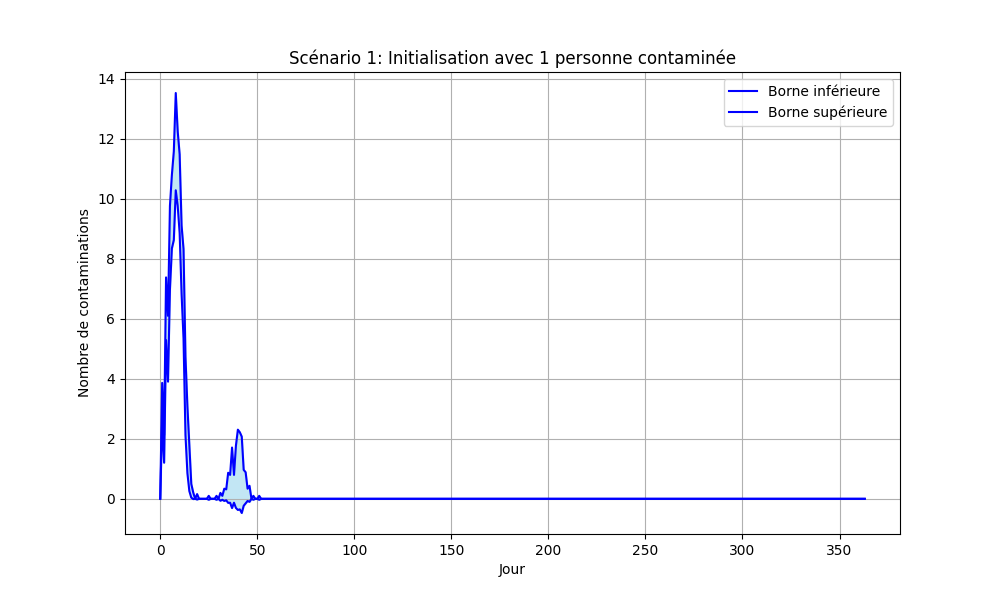
\includegraphics[width=0.9\textwidth]{graphiques/default/num_infect_init_1.png}
    \caption{default - num\_infect\_init\_1}
    \label{fig:default-num_infect_init_1}
\end{figure}

\begin{figure}[H]
    \centering
    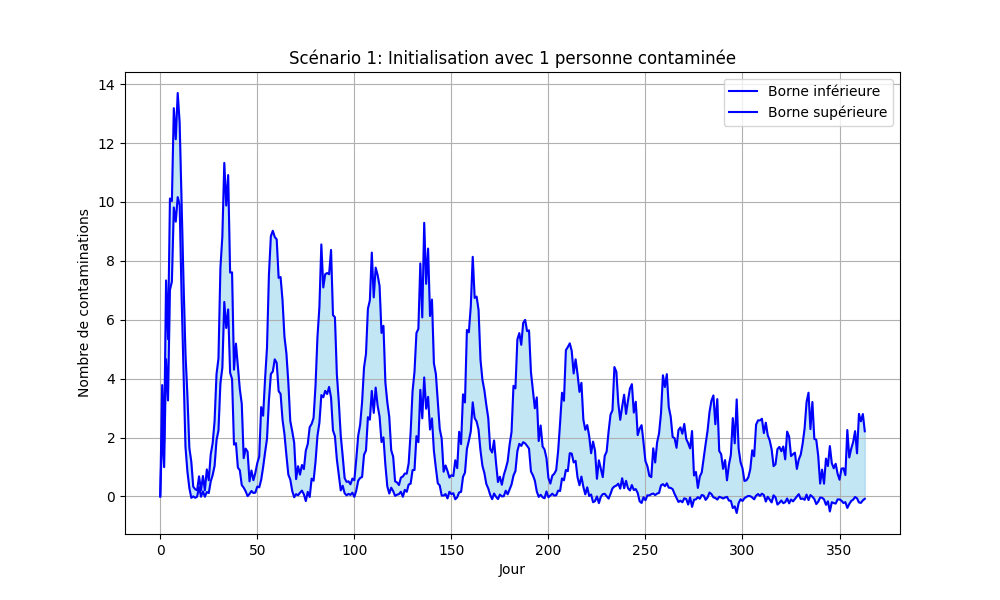
\includegraphics[width=0.9\textwidth]{graphiques/default-duree-immunite-10/num_infect_init_1.png}
    \caption{default-duree-immunite-10 - num\_infect\_init\_1}
    \label{fig:default-duree-immunite-10-num_infect_init_1}
\end{figure} 

\begin{figure}[H]
    \centering
    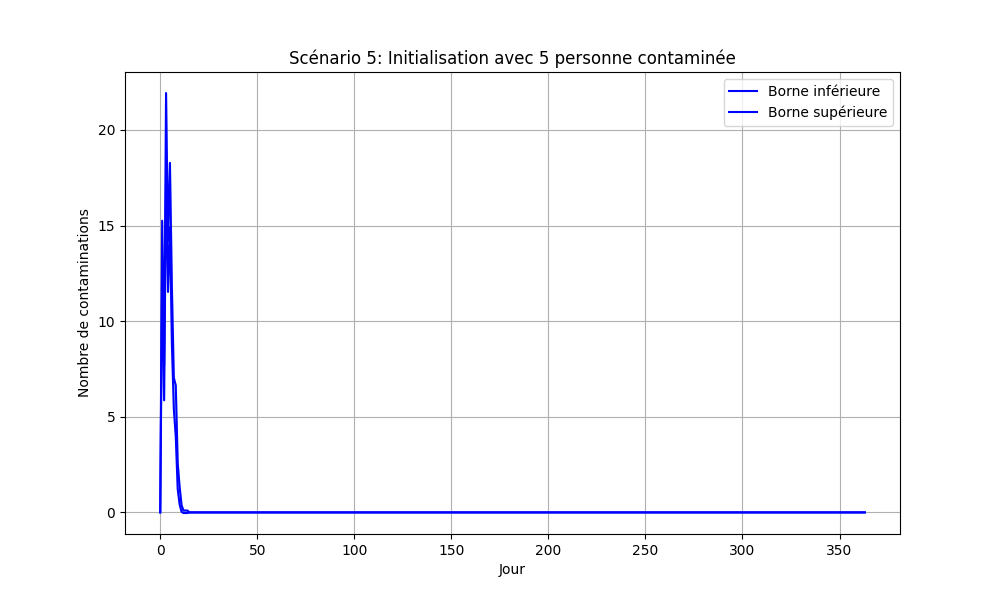
\includegraphics[width=0.9\textwidth]{graphiques/default-duree-immunite-10/num_infect_init_5.png}
    \caption{default-duree-immunite-10 - num\_infect\_init\_5}
    \label{fig:default-duree-immunite-10-num_infect_init_5}
\end{figure}

\begin{figure}[H]
    \centering
    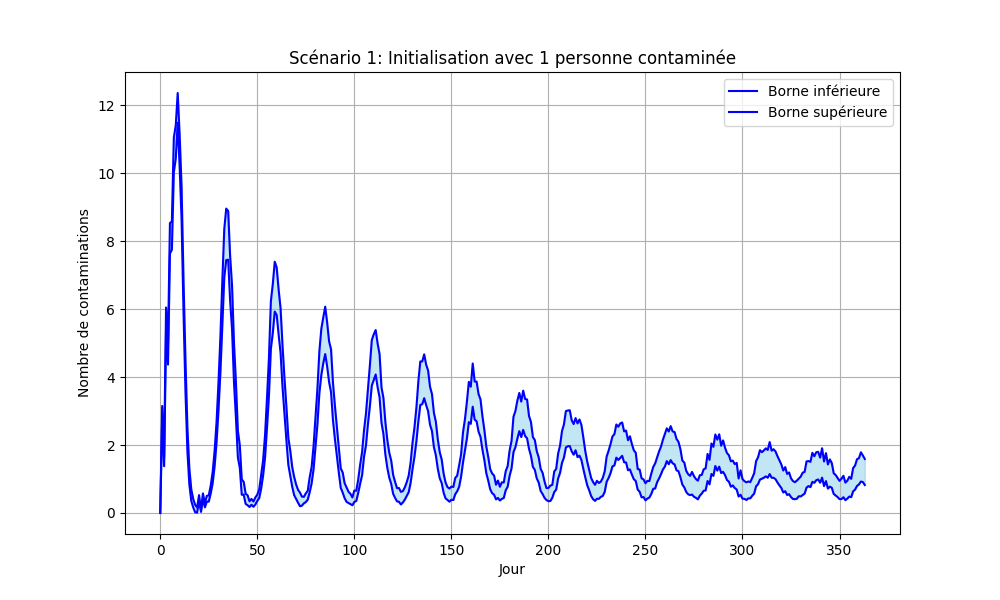
\includegraphics[width=0.9\textwidth]{graphiques/default-duree-immunite-10-replic-300/num_infect_init_1.png}
    \caption{default-duree-immunite-10-replic-300 - num\_infect\_init\_1}
    \label{fig:default-duree-immunite-10-replic-300-num_infect_init_1}
\end{figure}

\begin{figure}[H]
    \centering
    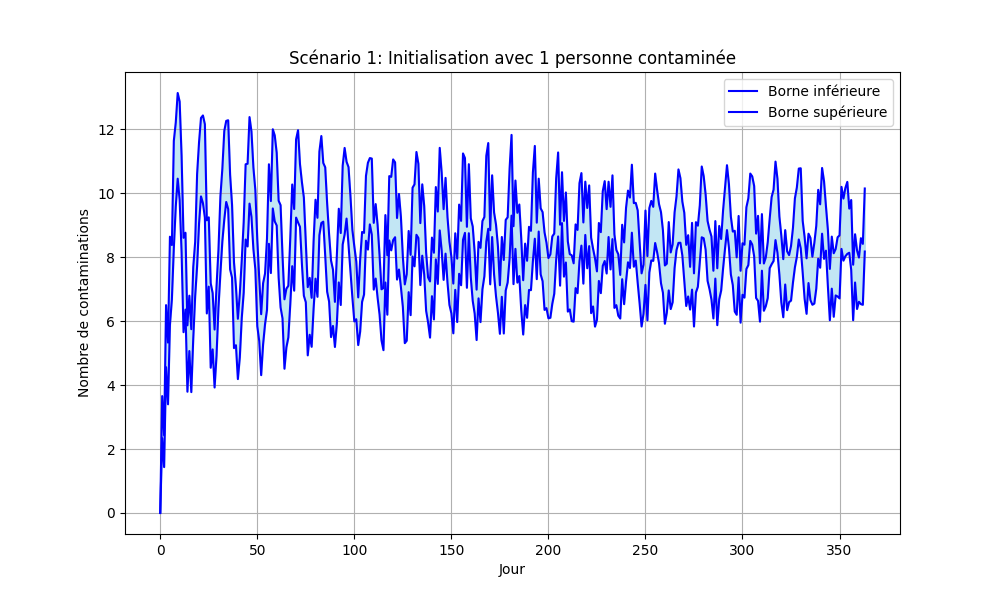
\includegraphics[width=0.9\textwidth]{graphiques/default-sans-immunite/num_infect_init_1.png}
    \caption{default-sans-immunite - num\_infect\_init\_1}
    \label{fig:default-sans-immunite-num_infect_init_1}
\end{figure}

\begin{figure}[H]
    \centering
    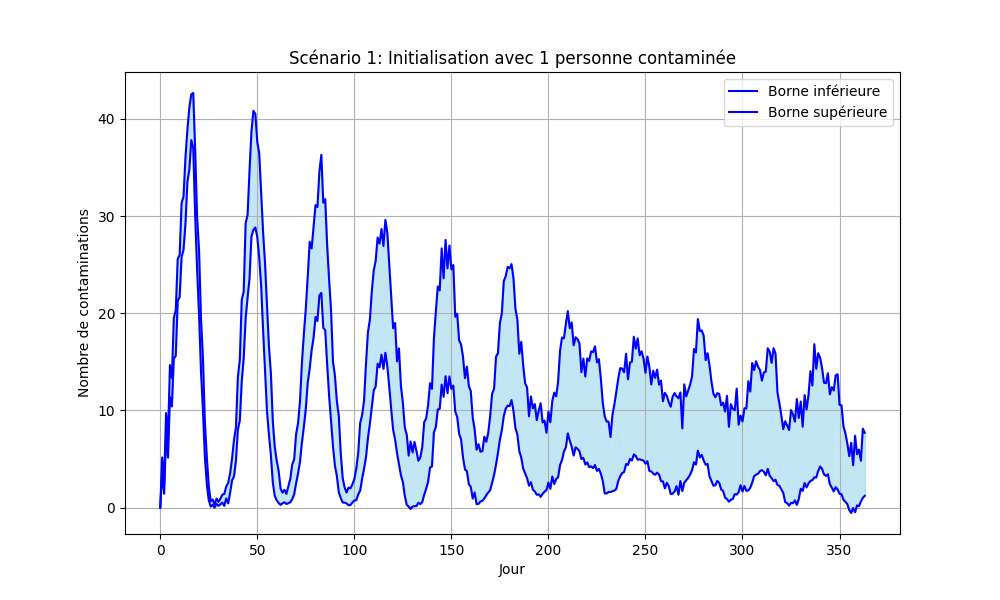
\includegraphics[width=0.9\textwidth]{graphiques/max/num_infect_init_1.png}
    \caption{max - num\_infect\_init\_1}
    \label{fig:max-num_infect_init_1}
\end{figure}

\begin{figure}[H]
    \centering
    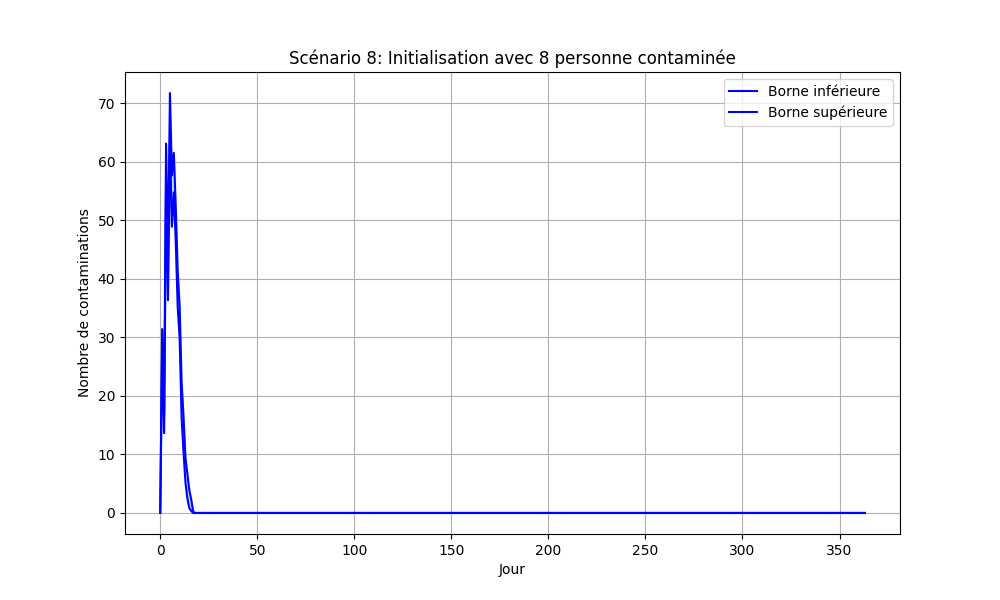
\includegraphics[width=0.9\textwidth]{graphiques/max/num_infect_init_8.png}
    \caption{max - num\_infect\_init\_8}
    \label{fig:max-num_infect_init_8}
\end{figure}

\begin{figure}[H]
    \centering
    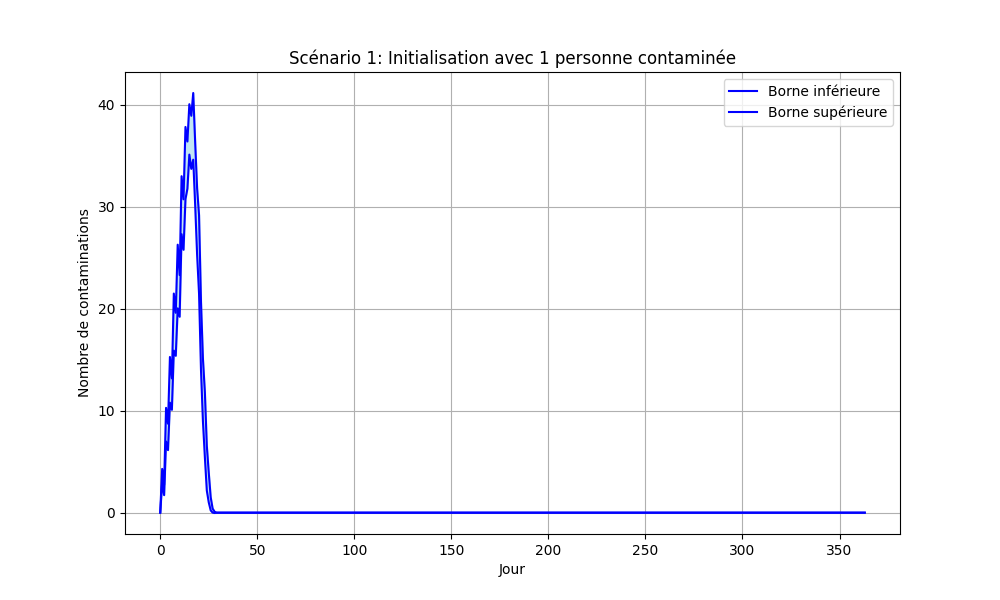
\includegraphics[width=0.9\textwidth]{graphiques/max-duree-immunite-30/num_infect_init_1.png}
    \caption{max-duree-immunite-30 - num\_infect\_init\_1}
    \label{fig:max-duree-immunite-30-num_infect_init_1}
\end{figure}

\newpage

\subsection{Script de création des graphiques}
\label{sec:script_graph}
Afin de m'aider à réaliser les graphiques utilisés dans cette rédaction, j'ai écrit un petit script en Python nommé \textbf{graphiques.py}, que vous pouvez retrouver dans le répertoire \textbf{redaction/}. 

Il est conçu pour générer un graphique représentant des intervalles de confiance à partir de données stockées dans un fichier CSV. Il fonctionne en important les packages \textbf{pandas} et \textbf{matplotlib.pyplot} qui servent respectivement à la manipulation de données et à la création de graphiques.\\

Le script prévoit l'usage d'arguments par ligne de commande. Seul le premier argument passé après le nom du script compte et est interprété comme le nom du répertoire dans lequel les fichiers des graphiques seront crées.

Des constantes sont définies pour indiquer où le script doit lire les fichiers CSV et où il doit créer les fichiers contenant les graphiques. Il lit donc les fichiers CSV crées par \textbf{stats\_sim} qui se situent dans le répertoire \textbf{out/} et dessine ses graphiques dans le répertoire \textbf{redaction/graphiques/}. L'argument passé par ligne de commande définit alors le sous-répertoire dans lequel les fichiers seront créés, tel que \textbf{redaction/graphiques/sous-repertoire/}.\\

Ensuite, le script définit et fait appel à une fonction nommée \textbf{draw}. Comme son nom l'indique, c'est elle qui est chargée de créer un fichier et de dessiner dedans un graphique correspondant à un fichier CSV. Elle prend comme paramètres un DataFrame (df) contenant les bornes inférieures et supérieures des intervalles de confiance, un titre pour le graphique, le chemin (path\_file) où enregistrer le graphique, et le nom du fichier (file\_name). Elle crée un graphique avec deux lignes (pour les bornes inférieure et supérieure) et une zone remplie entre elles, représentant les intervalles de confiance.

Le script fait appel à \textbf{draw} pour chaque fichier source CSV afin de créer un graphique par fichier source. Chaque appel est précédé par la création d'un DataFrame où les données de la première colonne du fichier csv sont contenues dans un champ correspondant à la borne inférieure et la seconde colonne dans un champ correspondant à la borde supérieure. L'appel se fait donc avec ce DataFrame en argument.

\newpage





\subsection{Crédits et liens externes}
Projet et rédaction réalisé par Léo Peyronnet
\begin{itemize}
\item Portfolio - \underline{\href{https://portfolio.leopeyronnet.fr/}{https://portfolio.leopeyronnet.fr/}}
\item Email - \underline{\href{mailto:peyronnet.leo@gmail.com}{peyronnet.leo@gmail.com}}\\
\end{itemize}

Le dépôt distant du projet est trouvable sur Github à cette adresse :

\underline{\href{https://github.com/LaiPe/sim-rhinite}{https://github.com/LaiPe/sim-rhinite}}

\end{document}
